% Membuat simbol flowchart (satu halaman per simbol), lalu diubah ke simbol-1.png ... simbol-6.png
\documentclass[tikz,border=2pt]{standalone}
\usetikzlibrary{shapes.geometric,shapes.symbols}
\tikzset{s/.style={draw,thick,minimum width=2.4cm,minimum height=1.1cm,inner sep=0pt}}
\begin{document}
% 1 proses
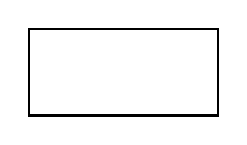
\begin{tikzpicture}\node[s,rectangle]{};\end{tikzpicture}
% 2 input/output
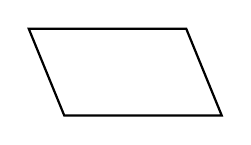
\begin{tikzpicture}\draw[thick](0.45,0)--(2.45,0)--(2.0,1.1)--(0,1.1)--cycle;\end{tikzpicture}
% 3 keputusan
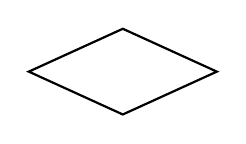
\begin{tikzpicture}\node[s,diamond,aspect=2.2]{};\end{tikzpicture}
% 4 basis data (drum horizontal)
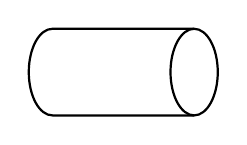
\begin{tikzpicture}
\draw[thick](0.3,0)--(2.1,0) arc(-90:90:0.3 and 0.55)--(0.3,1.1) arc(90:270:0.3 and 0.55);
\draw[thick](2.1,0) arc(-90:-270:0.3 and 0.55);
\end{tikzpicture}
% 5 dokumen / predefined
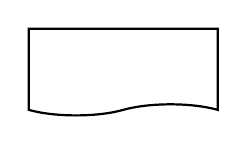
\begin{tikzpicture}\node[s,tape,tape bend top=none,tape bend height=4pt]{};\end{tikzpicture}
% 6 terminal
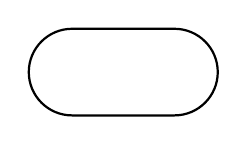
\begin{tikzpicture}\node[s,rectangle,rounded corners=0.55cm]{};\end{tikzpicture}
\end{document}
